\documentclass{article}
\usepackage{polski}
\usepackage[utf8]{inputenc}
\usepackage{float}
\usepackage{enumerate}

\title{Interpolacja funkcjami sklejanymi poprzez wyznaczenie
wartości drugich pochodnych w węzłach.
}
\author{Wiktoria Zaczyk}
\date{29.04.2021}

\usepackage{natbib}
\usepackage{graphicx}
\graphicspath{ {./images/} }

\begin{document}

\maketitle

\section{Wstęp teoretyczny}

\newline\newline
\textbf{Interpolacja}:
\newline
Metoda numeryczna przybliżania funkcji interpolowanej w zadanym przedziale 
funkcją interpolującą, która w punktach zwanych węzłami interpolacji przyjmuje wartości takie 
same jak przybliżana funkcja.
\newline

\textbf{Funkcja sklejana}
\newline
W metodzie tej stosowane są funkcje zdefiniowane jako wielomiany niskiego stopnia osobno dla każdego podprzedziału pomiędzy sąsiednimi węzłami interpolacyjnymi. 
\newline\newline
\textbf{Interpolacja funkcjami sklejanymi}
W przedziale [a,b] mamy n+1 punktów, które dzielą go na n przedziałów $[x_i, x_i_+_1]$. Funkcja sklejana S jest m stopnia i spełnia warunki: 

\begin{enumerate}
\item S(x) jest wielomianem stopnia conajwyżej m na każdym przedziale $(x_i, x_i_+_1)$, i=0,1,...,n-1
\item $S(x) \in C^m$
\end{enumerate}
Funkcja jest kombinacją liniową elementów bazy \{$S_i(x)$\}:  \[ s(x)= \sum_{i=0}^{n-1} c_is_i(x), x \in [a,b] \]
Aby nasza interpolacja była poprawna szukamy funkcji: 
\newline
$m_j=s^2(x_j), j=0,1,...,n$
\newline\newline
Aby wyznaczyć pochodne w węzłach, należy rozwiązać układ równań liniowych: $A \overrightarrow{m} = \overrightarrow{d}$, którego generatorem jest: $\mu_i m_i_-_1+2m_i +\lambda_im_i_+_1=d_i$
\newline

Po wprowadzeniu warunków brzegowych do układu równań, przyjmuje on postać:

\begin{center}

\left[ \begin{array}{cccccc}
1 & 0 & 0 & \cdots & \cdots & 0 \\
\mu_1 & 2 & \lambda_1 & \cdots & \cdots & 0\\
0 &  \mu_2 & 2 & \lambda_2 & \cdots & 0\\
\vdots & & & \ddots & & \vdots \\
0 & \cdots &\cdots & \mu_n_-_2 & 2 & \lambda_n_-_2\\
0 & \cdots &\cdots & 0 & 0 & 1
\end{array} \right] 
\left[ \begin{array}{c}
m_0\\
m_1\\
\vdots\\
\vdots\\
m_n_-_2\\
m_n_-_1\\
\end{array} \right]
\mathbf{}=
\left[ \begin{array}{c}
\alpha \\
d_1\\
\vdots\\
\vdots\\
d_n_-_2\\
\beta
\end{array} \right]
\end{center}
\newline\newline
gdzie: 
\begin{itemize}
\item $\lambda_i=\frac{h_i_+_1}{h_i+h_i_+_1}$, \item $\mu_i=1-\lambda_i$ 
\item $d_i=\frac{6}{h_i+h_i_+_1}(\frac{y_i_+_1-y_i}{h_i_+_1}-\frac{y_i-y_i_-_1}{h_i})$
\item $h_i=x_i-x_i_-_1$
\end{itemize}
\newline\newline
Po jego rozwiązaniu jesteśmy w stanie wyznaczyć wartości funkcji z poniższego wzoru:
$s_i_-_1(x)=m_i_-_i\frac{(x_i-x)^3}{6\cdoth_i}+m_i \frac{(x-x_i_-_1)^3}{6\cdoth_i}+A_i(x-x_i_-_1)+B_i$
\newline\newline 
\textbf{Efekt Rungego}:
\newline
Mówimy o nim gdy zadanie jest źle uwarunkowane, czyli kiedy zaczynają występować niedopasowania wielomianu interpolacyjnego na krańcach przedziału w wyniku zwiększnia liczby wezłów. Wynika to z oscylacji wielomianów wyższych rzędów. W celu zapobiegnięcia tego efektu stossuje się metody optymalizujące położenia węzłów.

\section{Cel zadania}
Na ósmych zajęciach zajęliśmy się interpolacją funkcjami sklejonymi poprzez wyznaczanie drugiej pochodnej w węzłach dla funkcji $f_1(x)=\frac{1}{1+x^2}$ oraz $f_2(x)=cos(2x)$ w przedziale $x\in[-5,5]$ dla liczby węzłów n = 5, 8, 21. Dodatkowo dla pierwszej funkcji oraz n = 10 węzłów wyznaczyliśmy wartości drugich pochodnych i porównaliśmy je z "dokładniejszymi" wartościami liczonymi zgodnie z wzorem: $\frac{d^2f}{dx^2}\approx \frac{f(x-\delta x)-2f(x)+f(x+\delta x)}{(\delta x)^2}$

\newpage
\section{Wyniki}
I. Wykresy funkcji $f_1=\frac{1}{1+x^2}$
\begin{figure}[h!]
\centering
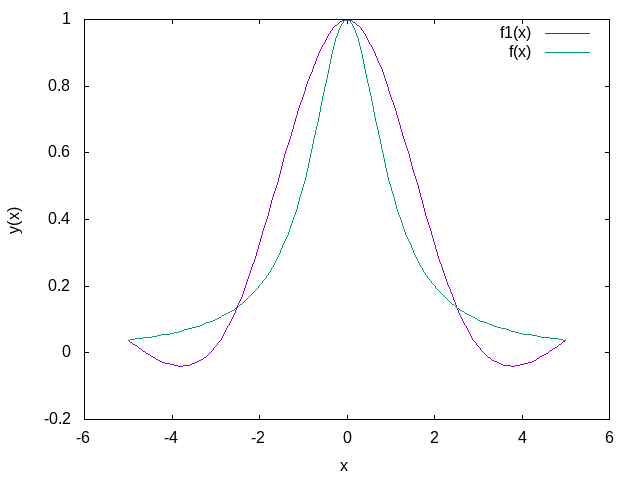
\includegraphics[width=10cm]{f1_5.png}
\caption{Wykres funkcji $f_1$ oraz jej interpolacji dla liczby węzłów n=5}
\label{fig:obrazek f1_5}
\end{figure}

\begin{figure}[h!]
\centering
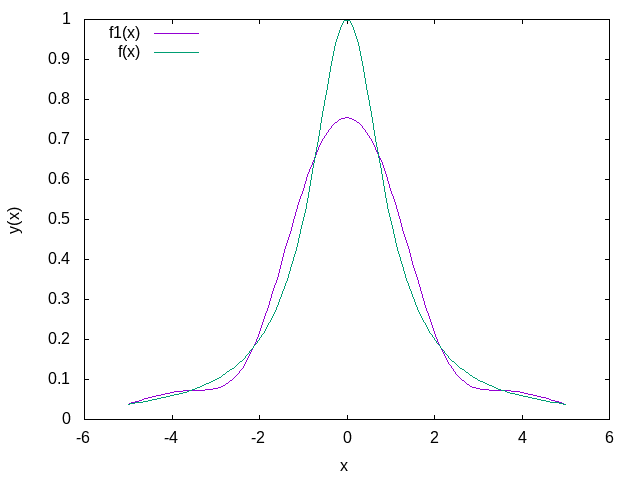
\includegraphics[width=10cm]{f1_8.png}
\caption{Wykres funkcji $f_1$ oraz jej interpolacji dla liczby węzłów n=8}
\label{fig:obrazek f1_8}
\end{figure}

\begin{figure}[h!]
\centering
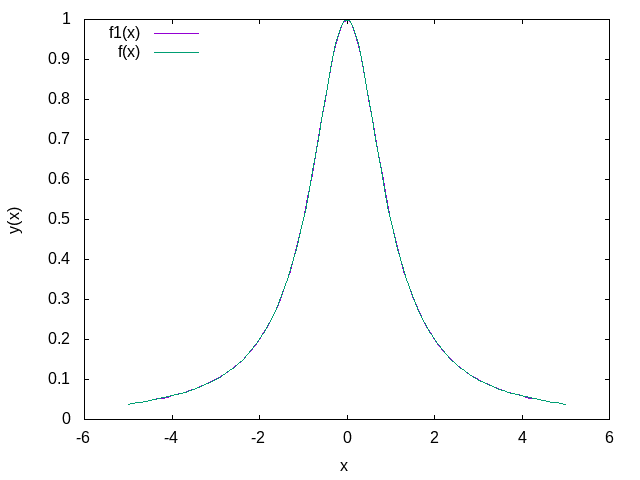
\includegraphics[width=10cm]{f1_21.png}
\caption{Wykres funkcji $f_1$ oraz jej interpolacji dla liczby węzłów n=21}
\label{fig:obrazek f1_21}
\end{figure}

Jak widać dla funkcji $f_1$, im większe jest n, tym bardziej dokładne jest dopasowanie interpolacji do funkcji.
\newpage
II. Wykresy funkcji $f_2=cos(2\cdot x)$
\begin{figure}[h!]
\centering
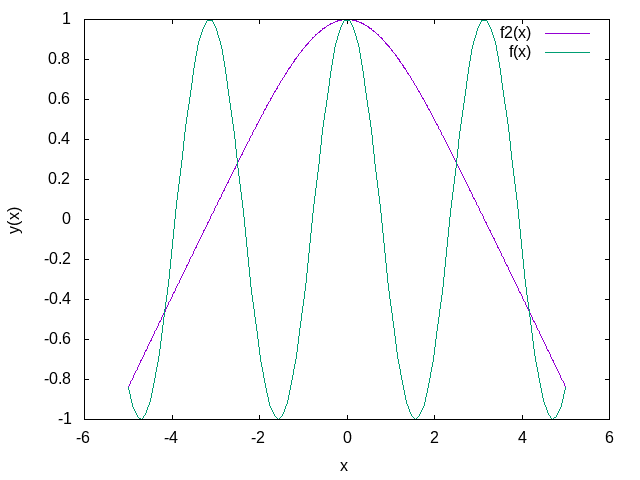
\includegraphics[width=10cm]{f2_5.png}
\caption{Wykres funkcji $f_2$ oraz jej interpolacji dla liczby węzłów n=5}
\label{fig:obrazek f2_5}
\end{figure}

\begin{figure}[h!]
\centering
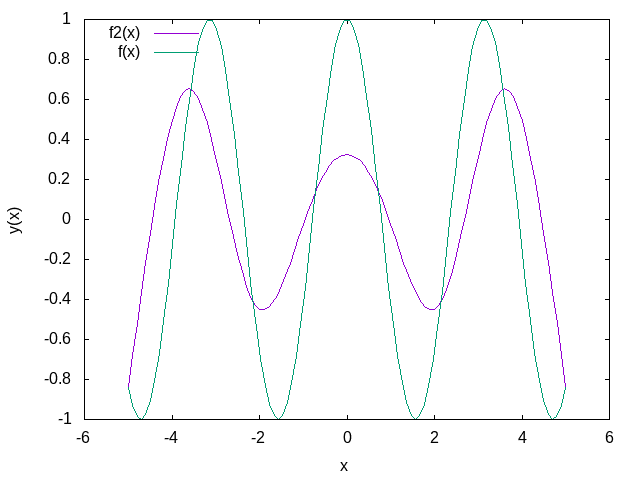
\includegraphics[width=10cm]{f2_8.png}
\caption{Wykres funkcji $f_2$ oraz jej interpolacji dla liczby węzłów n=8}
\label{fig:obrazek f2_8}
\end{figure}

\begin{figure}[h!]
\centering
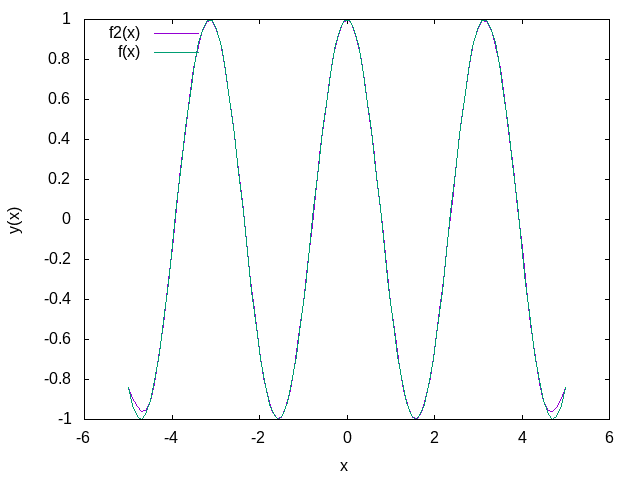
\includegraphics[width=10cm]{f2_21.png}
\caption{Wykres funkcji $f_2$ oraz jej interpolacji dla liczby węzłów n=21}
\label{fig:obrazek f2_21}
\end{figure}
\newpage
Jak widać dla funkcji $f_2$, dla n = 5 interpolacja jest bardzo niedokładna, natomiast przy zwiększeniu liczby węzłów sytuacja się polepsza, i dla n = 21 dopasowanie pokrywa się z funkcją

\begin{figure}[h!]
\centering
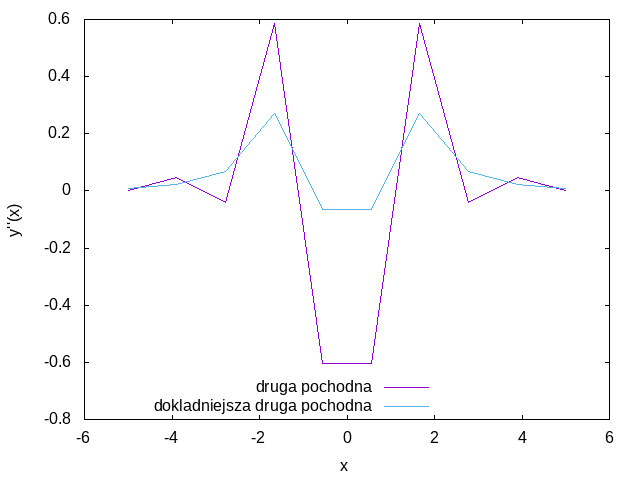
\includegraphics[width=10cm]{pochodne.png}
\caption{Wykres wartości drugich pochodnych funkcji $f_1$ w zależności od położenia węzłów, pokazujący 
porównanie obu sposobów obliczania drugich pochodnych}
\label{fig:obrazek pochodne}
\end{figure}
\newpage
Jak widać, wykres wyznaczonych pochodnych zachowuje kształt wykresu ich dokładnych 
wartości, jednak im bliżej środka wykresu - tym większa jest różnica między wykresami.


\section{Wnioski}
Wyniki dla odpowiednio dużej liczby węzłów pokrywają się niemal idealnie z interpolowaną funkcją. Nie było  efektu Rungego na granicach przedziałów interpolacji, jednak można zauważyć, że właśnie na granicach przedziałów funkcja interpolująca najbardziej odstaje od funkcji interpolowanej. Porównanie wykresów funkcji bardzo dokładnie obrazuje jaką ilość węzłów należy zastosować dla danej funkcji, oraz to, czy metoda jest akceptowalna.
\end{document}